\section{Local Stores in Dafny}

\subsection{Local Store ADT}

Figure~\ref{fig1} shows Utting's specification for an ADT for a local
store \cite{utting1995,utting1998}.  The store ADT is essentially a
map from pointers (\textit{Ptr}) to values (\textit{Val}).

\begin{figure}[t]
\centering
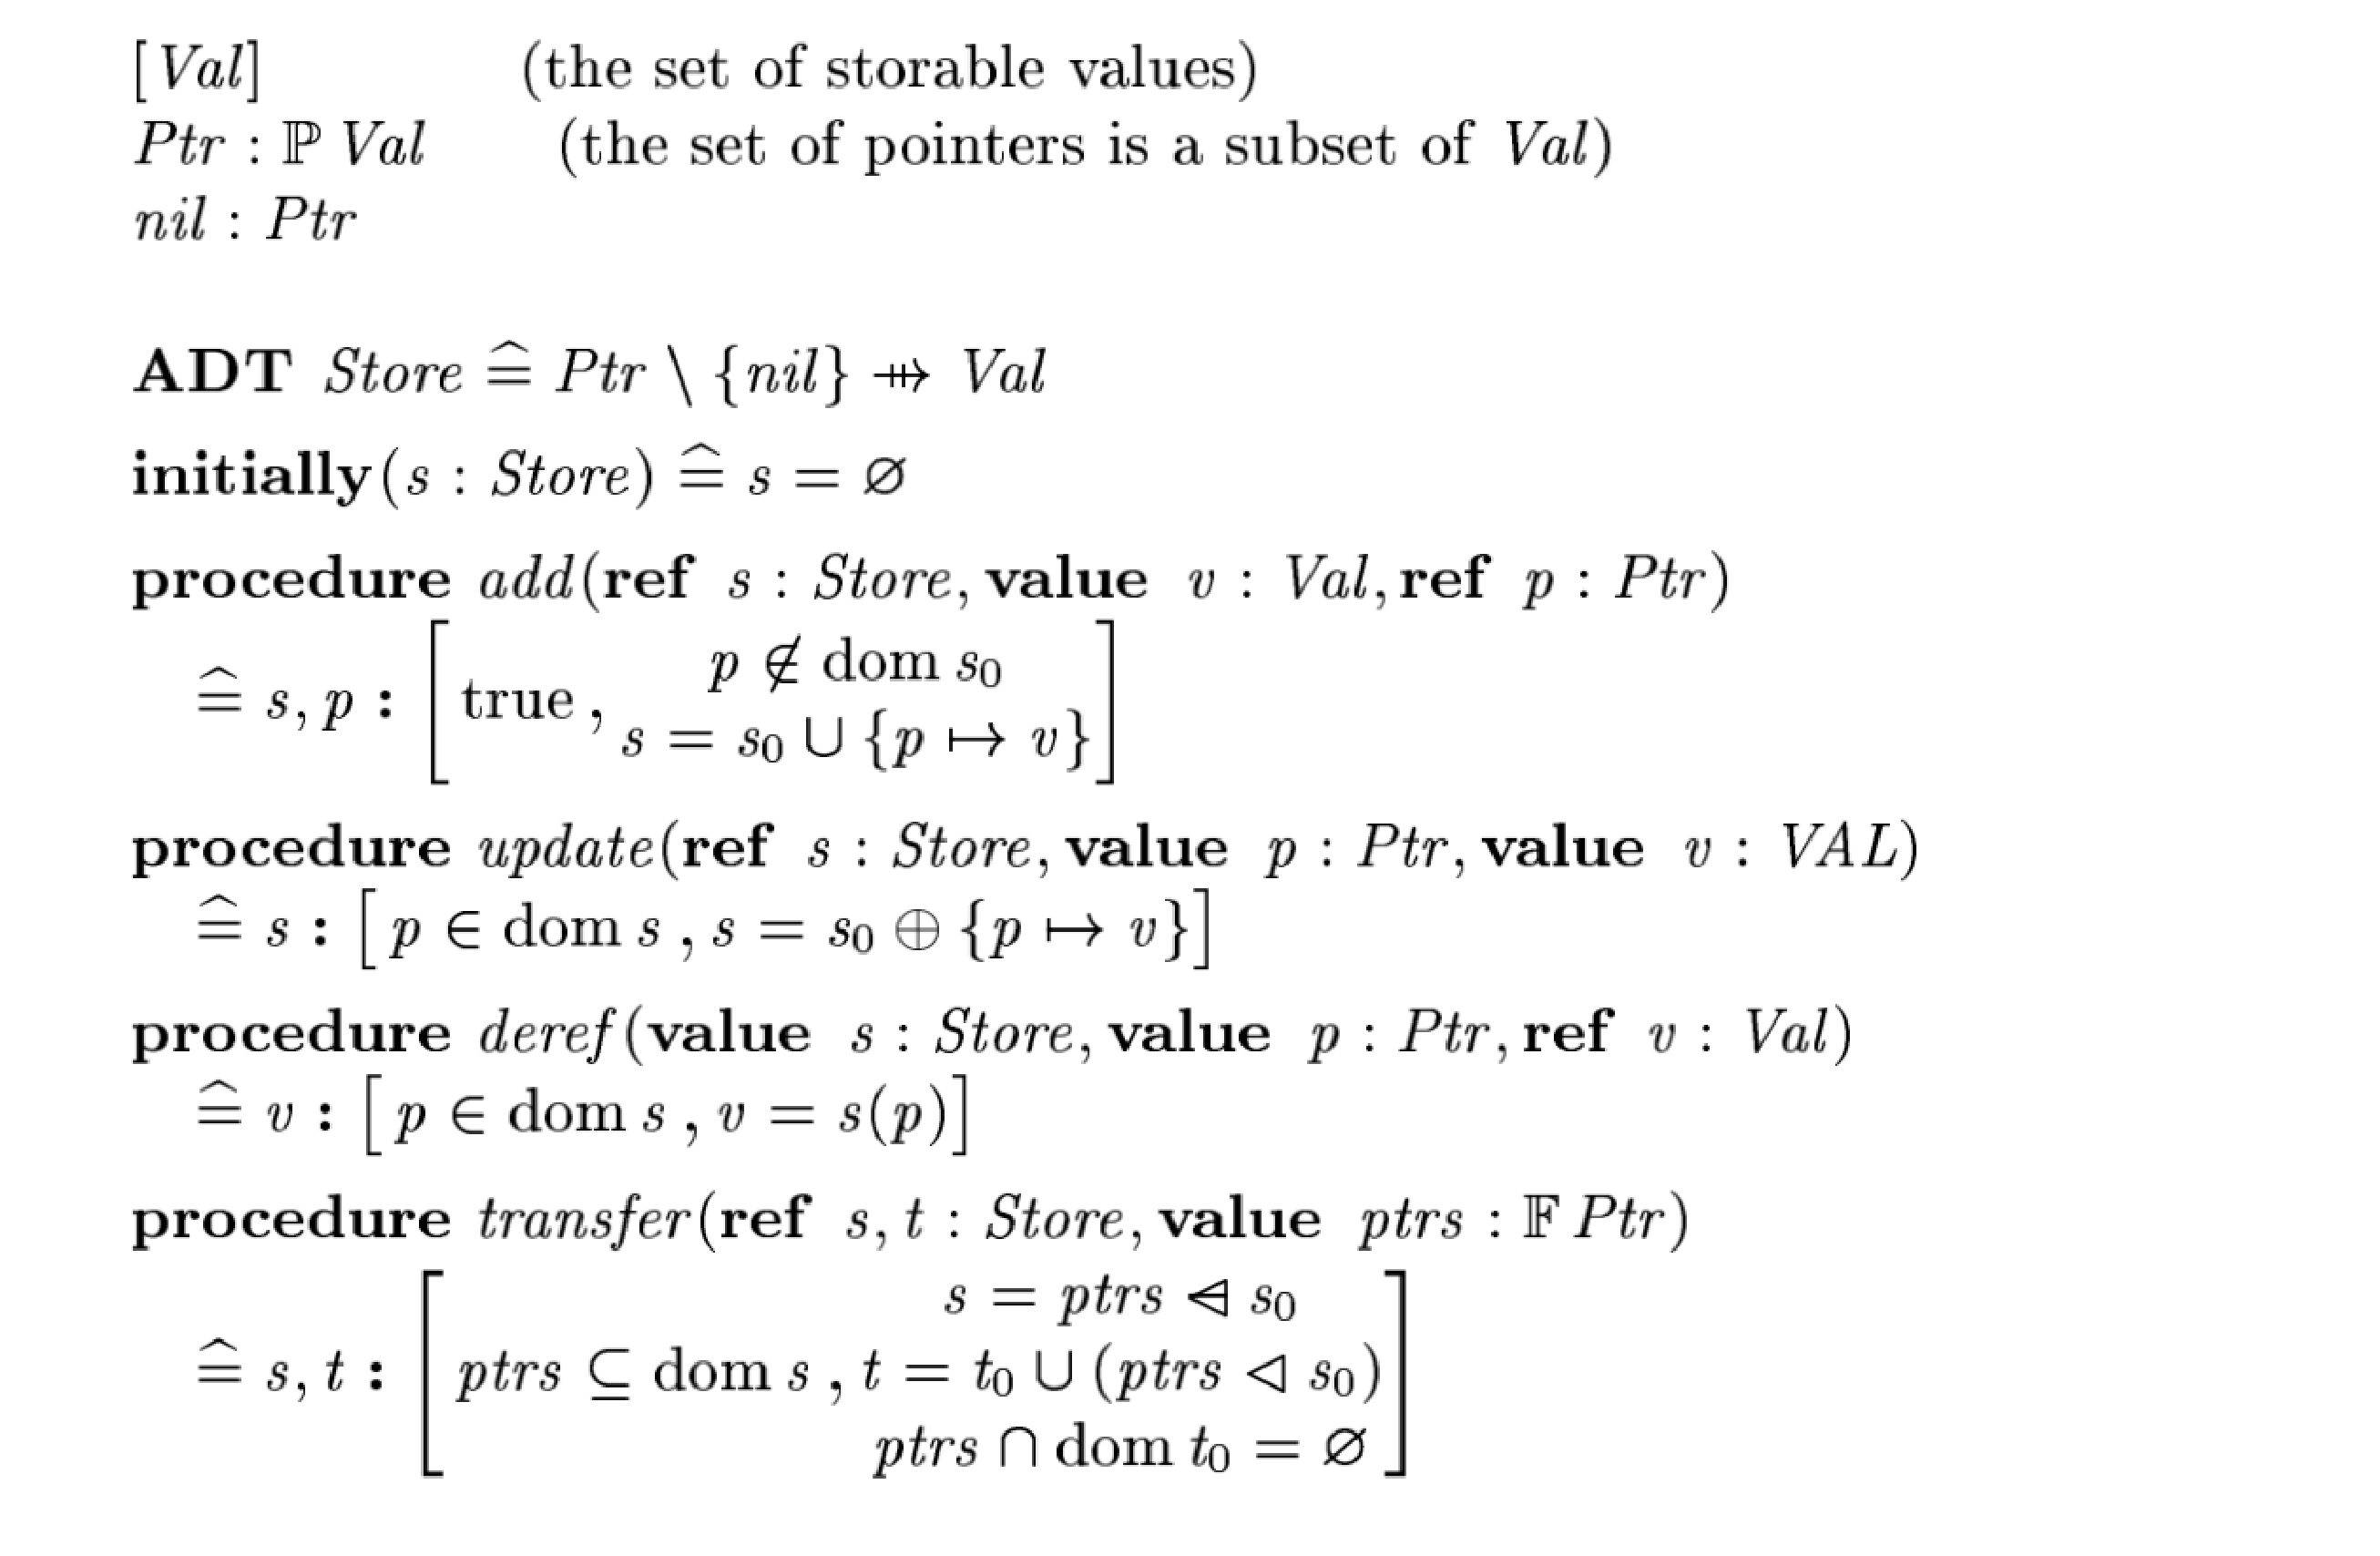
\includegraphics[width=0.5\textwidth]{LocalStoreADT.pdf}
\Description{Z specification for Local Store ADT}
\caption{Z specification for Local Store ADT, from
  \citet{utting1995,utting1998}}
\label{fig1}
\end{figure}

The ADT has five methods:
\begin{itemize}
\item \textbf{add} in a new pointer to value mapping.
\item \textbf{update} an existing mapping
\item \textbf{deref}erence a pointer, returning the corresponding
  value.
\item \textbf{transfer} a pointer from one store into another.
\end{itemize}

We could convert the Z ADT to Dafny quite straightforwardly (see
Figure~\ref{fig2}) but unfortunately this can't really be used to
emulate local stores.  To see why, consider the signature of the
``\textbf{deref}'' method. This returns the dereferenced value of
``$v$'' --- however Dafny doesn't make it possible to place any
further restrictions on the use -- the result is no longer tied to the
local store in any way.

\begin{figure}[htb]
\centering
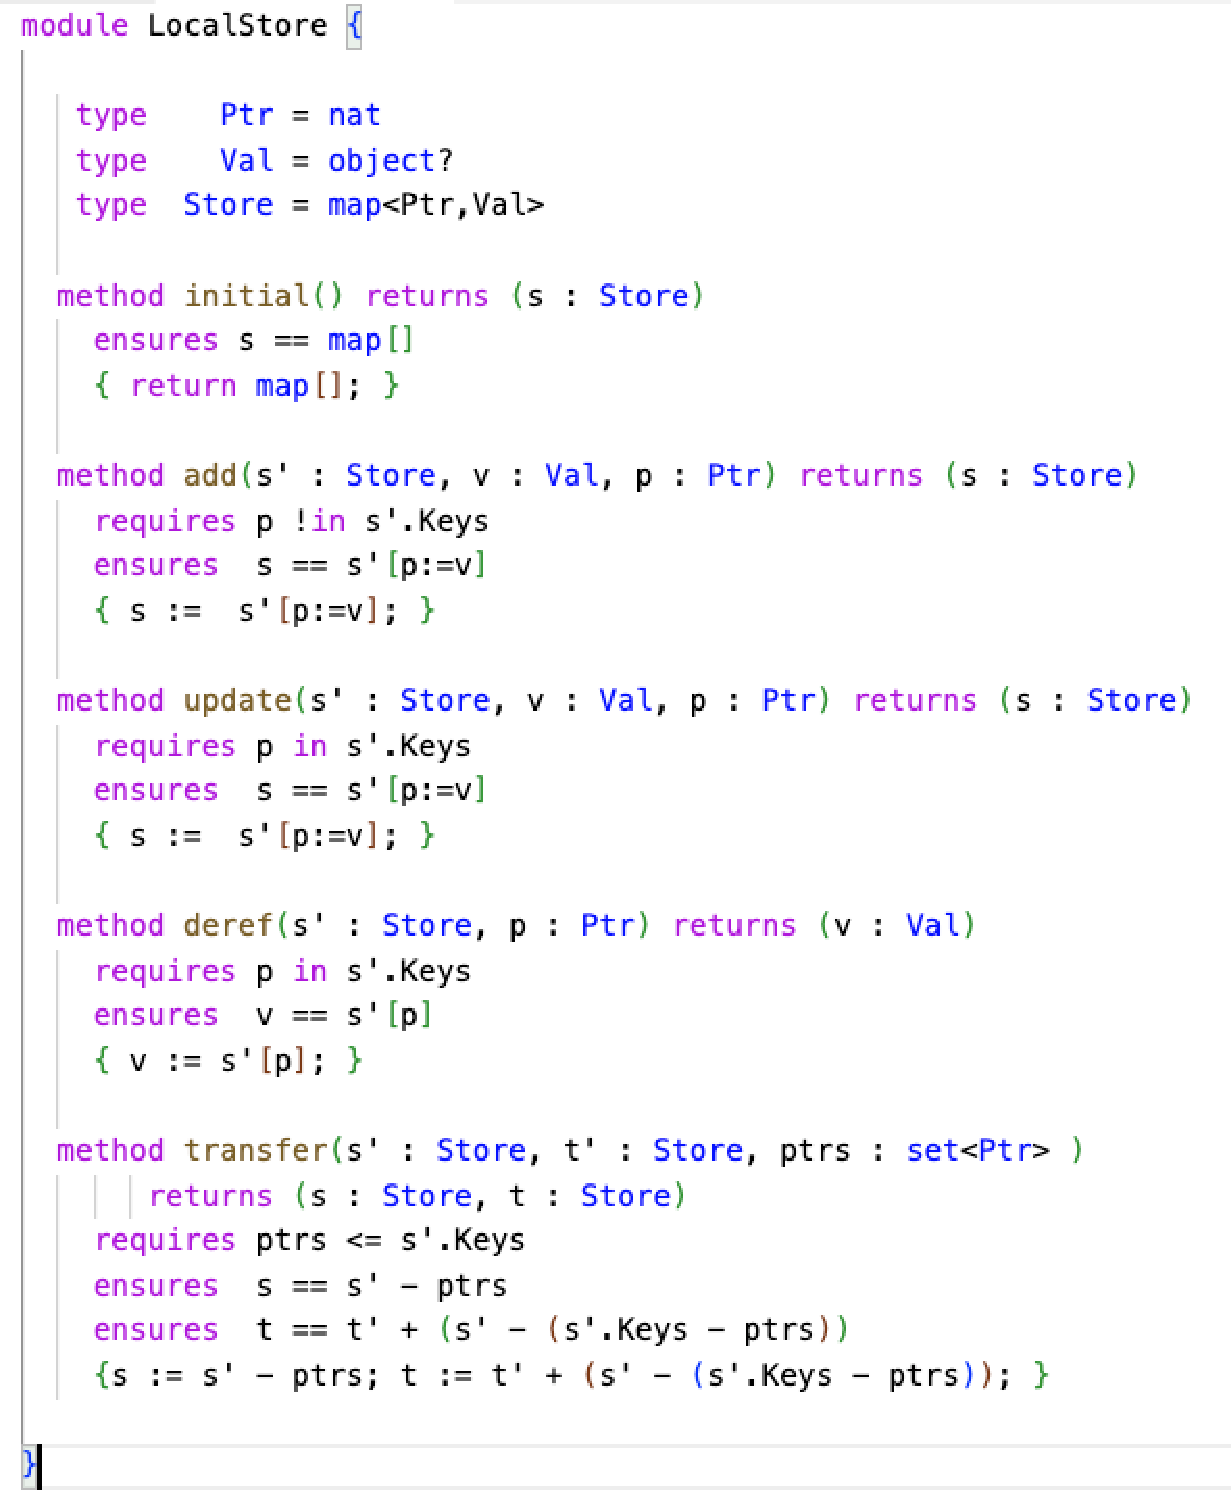
\includegraphics[width=0.5\textwidth]{LocalStoreDafny.pdf}
\Description{Dafny Local Store ADT}
\caption{Dafny Local Store ADT}
\label{fig2}
\end{figure}




\subsection{Local Stores and Objects}

Based on our work-in-progress of models of ownership in
programming languages \cite{dafnydala-ftfjp2024}, we surmised the
problem was that the Dafny objects in the store were not tied tightly
enough to the store to which they belonged. 

The core of our ownership model is the Dafny class \lstinline+Object+
(note that while \lstinline+object+ is a reserved word in Dafny,
\lstinline+Object+ is not --- neither is \lstinline+Class+)). We will
reuse the design of class Object \lstinline+Object+ to model an object
allocated in a local store. In particular, we have an
``\lstinline+owner+'' field in \lstinline+Object+ which holds the
local store in which the object is allocated -- set up when the Object
is allocated.

\begin{lstlisting}
  class Object {  
      const owner : Store
 
    constructor(oo : Store) 
      ensures  owner  == oo
      { 
        owner := r; 
        ...
\end{lstlisting}

Programmers must ensure objects they wish to use in local stores
are instances of classes that extend our \lstinline+Object+,
rather than Dafny's \lstinline+object+. Once that's done
they can use Dafny assertions to constrain object references
to refer only to instances within a particular store, or the same
store as some other object.  Consider the following example:

\begin{lstlisting}
  method disjoint(a : Object, b : Object)
     requires a.owner != b.owner
     modifies a`counter
     ensures  a.counter >  old(a.counter)
     ensures  b.counter == old(b.counter)
     {
       a.thump();
      }
\end{lstlisting}

\noindent here, the two arguments a and b are in two different local stores 
they must be two different objects. As a result, if a is modified,
we can still establish that b is not modified: both postconditions can
be verified.  Without the precondition saying the owning local stores
are disjoint, the postcondition ensuring that \lstinline+b.counter+  is
unchanged even though  \lstinline+a.counter+ most certainly is changed
could not be verified.

The result is not that dissimilar to programming in a
language with explicit region allocation: we can allocate a store,
then allocate objects with the store, then use those objects.

\begin{lstlisting}
  method Main()
     {
       var global : Store = new Store();
       ...
       while (stream.notEmpty)
       {
         var local : Store = new Store();
         process(stream.current, within:=local);
         stream.advance();
       }
     }
\end{lstlisting}

The catch is that, unlike e.g.\ Rust, Euler, Cyclone, or Linear Dafny,
there's no obvious way to constrain the use of the objects allocated
in the store. Although in the code above, the \lstinline+local+ store
appears to be scoped within the \lstinline+global+ store, and that
would be the case in Rust, say, our basic Dafny implementation doesn't
enforce that constraint.

\subsection{Nested Local Stores}

There are two issues that must be resolved:
\begin{itemize}
\item a nesting relationship needs to be established between stores
\item types and assertions need to be aware of that relationship
\end{itemize}

\noindent Establishing the nesting relationship is relatively straightforward: 
we extend stores to say which other stores they are nested within,
and provide an API such \lstinline+inside(part, whole)+ that determines
if one store is inside another:

\begin{lstlisting}
    var global : Store = new Store();
    ...
    ...
    var local : Store = new Store(global);
    ...
    var localObject := new Object(local);

    assert inside(local, global); //should verify
    assert inside(global, local); //should not verify
\end{lstlisting}

While we can use the API to verify nesting relationships, we again
have to do this explicitly --- just as we have to bind instances
explicitly into a local store.  Then, objects should be constrained by
the store structure so e.g.\ a global object cannot have incoming
pointers into nested local storage.  Our programming language heap
model addresses this by implementing object fields directly in a
hashtable \cite{dafnydala-ftfjp2024}, rather than by reusing Dafny's
own fields:
\pagebreak[3]

\begin{lstlisting}
  class Object {  
      const store : Store;
      var fields : map<string,Object>;  
\end{lstlisting}

Using this, we can e.g. place constraints on which references are
permitted:


\begin{lstlisting}
    predicate AllOutgoingRefsDala()
      reads this`fields
        { forall n <- fields ::
            DalaRefOK(kind, fields[n].kind) }
\end{lstlisting}

To gain maximum advantage of local stores, either some kind of
reflexive access to object's fields would be required, or a Dafny
plugin could be written to extend the compiler to undertake the
checks. Again referring back to Euler, a plugin to implement the
rule that stores may not be components of other stores, and may only
be passed as var parameters (i.e. only up the stack,  but not returned
down it should be straightforward. Establishing proof obligations
that an object can only be accessed when it's store is in scope
appears no harder in principle than ensuring that keys must be in a
Dafny map before they can be accessed. 


\subsection{From Stores to Owners}

Dynamic Frames, like desmesnes before them, require objects e.g. to
delineate their representations for framing, typically by writing a
function (desmesnes \cite{wills91} or original dynamic frames
\cite{dynamic-frames-fm2006}, or by updating a data structure
explicitly --- Dafny's \lstinline+Repr+ is a field, not a function.
For example, a lookup table implemented by two parallel arrays
would need to set \lstinline+Repr+ explicitly in its constructor:

\begin{lstlisting}
class Table<Data> {
  ghost var Repr: set<object>

  var keys : array<int>
  var values : array<Option<Data>>

  var size : nat
  var capacity : nat
    
  constructor (initial : nat)
    requires initial > 0
    ensures Valid() && fresh(Repr)
    {   
       capacity := initial;
       new;
       keys := new int[capacity];
       values := new Option<Data>[capacity](_ => None);

       size := 0;
       Repr := { this, keys, values };
     }
 
\end{lstlisting}


\noindent and then update \lstinline+Repr+
after every method that changes the representation:

\begin{lstlisting}
method Expand()
    requires Valid()
    modifies this`keys, this`values, this`capacity, this`Repr
    ensures Valid() && fresh(Repr - old(Repr))
    ensures size == old(size)
    ensures capacity == old(capacity) * 2
   {
       keys := new int[capacity * 2] //...
       values := new Option<Data>[capacity * 2] //...
       capacity := capacity * 2;

       Repr := { this, keys, values }; 
\end{lstlisting}


\noindent In contrast, a desmesnes function would only need to be
defined once, and could just be called whenever the footprint of the
representation needed to be determined:

\begin{lstlisting}
function desmesnes() : set<object> {{this,keys,values}} 
\end{lstlisting}


We hypothesize that ownership offered by local stores can reduce the
effort further: rather than defining either a \lstinline+Repr+ data
structure or a desmesnes function, programmers could simply allocate
an object's representation within a local store for that purpose:

\begin{lstlisting}
class Table<Data> {
  ghost var Repr: Store

  var keys : array<int>
  var values : array<Option<Data>>

  var size : nat
  var capacity : nat
    
  constructor (initial : nat)
    requires initial > 0
    ensures Valid()
    {  
       const ReprStore := new Store(this);
      
       capacity := initial;
       new;
       keys := new array<int>(capacity, ReprStore);
       values := new Option<Data>(capacity, ReprStore);

       size := 0;
     }
 
\end{lstlisting}

\noindent or one step further, providing every object with a store,
and allowing types or variables to be annotated, we could arrive at
something much close to Ownership Types \cite{noble_flexible_1998} or Rust:

\begin{lstlisting}
class Table<Data> {
  var {:rep}  keys : array<int>
  var {:rep} values : array<Option<Data>>

  var size : nat
  var capacity : nat
    
  constructor (initial : nat)
    requires initial > 0
    ensures Valid()
    {  
       capacity := initial;
       new;
       keys := new {:rep} array<int>(capacity);
       values := new {:rep} Option<Data>(capacity);

       size := 0;
     }
 
\end{lstlisting}





%% we have shown how
%% Dafny's object model can be extended to incorporate local stores into
%% object implementations, and how we can use those local stores to
%% support reasoning about aliasing.


%% The key fields of an \lstinline+Object+ are the \lstinline+kind+,
%% the \lstinline+fieldKinds+, and the object's \lstinline+fields+.

%% The Dala model is fundamentally untyped, in that it is not set up to track e.g.\ the differences between a Point and a Rectangle class. Rather the 
%% \lstinline+kind+ field captures the object's ownership capability: \
%% Immutable (\lstinline+Imm+),
%% Isolated (\lstinline+Iso+),
%% or Local (\lstinline+Mut+, originally mutable).

%% \begin{lstlisting}
%%     datatype Kind = Imm | Iso | Mut 
%% \end{lstlisting}

%% We treat Dala's ownership capabilities more like meta-types rather that traditional types:
%% they are close to what are often called
%% "reference capabilities"~\cite{caps-ecoop2001,castegren_reference_2016} but 
%% apply to individual objects, rather than each reference to an object.
%% In many languages capabilities manifest as additional keywords or attributes attached to variables that control how those variables may be used --- i.e.\ how they relate to heap topologies and their evolution. In the Dafny code example above, the difference between \lstinline+const+ and \lstinline+var+ could potentially be considered different kinds of reference capability.

%% In Dala, then, an object's \lstinline+kind+ is the kind (ownership capability) of that object. The \lstinline+fields+ map models object' fields as a map between field names ( strings) and the \lstinline+Object+s stored in each field; the \lstinline+fieldKinds+ map likewise gives the declared kind for each field.

%% Dafny \lstinline+map+s are immutable --- only Dafny \lstinline+class+ instances are mutable: only \lstinline+var+ fields of classes; \lstinline+const+ fields are, well, constant.  What this means is that while the values stored by Dala objects' fields can change (or rather, while our model permits them to change) the kinds of each field of each instance of that Dahlia class are fixed.

%% The \lstinline+Object+ class contains a number of helper functions, such as \lstinline+outgoing()+, which returns all outgoing references from an object, abstracting away field names; and \lstinline+fieldNames()+ which returns the names of fields, without their values. 

%% Finally, the class contains a Dafny invariant, represented as a Dafny predicate conventionally called \lstinline+Valid()+, which ensures the validity of each individual object.  This predicate is typically defined as a conjunction of smaller invariants that must usually be adjusted to suit the particular heap being modelled. A minimal validity predicate would be something like this: 

%% \begin{lstlisting}
%%     predicate Valid()
%%     reads this`fields
%%       {  AllFieldsAreDeclared() 
%%         && AllFieldsConsistentWithDclrn() }
%% \end{lstlisting}

%% \noindent saying that all fields (entries in the \lstinline+fields+) must have a corresponding entry in the \lstinline+fieldKinds+, and that the kind of object stored in a field must match the kind expected for that field.  These are defined by auxiliary predicates: 

%% \begin{lstlisting}
%%     predicate AllFieldsAreDeclared() 
%%       reads this`fields 
%%         { fields.Keys <=set  fieldKinds.Keys }

%%     predicate AllFieldsConsistentWithDclrn() 
%%       requires AllFieldsAreDeclared()
%%       reads this`fields 
%%         { forall n <- fields ::
%%             fieldKinds[n] == fields[n].kind }
%% \end{lstlisting}



%% \subsection{Dala Heaps}

%% The other main structure in Dala is the heap itself, modelled by the eponymous \lstinline+Heap+ class. The Heap class looks trivial --- a Dala heap is just a set of Dala objects:

%% \begin{lstlisting}
%% class Heap {
%%   var objects : set<Object>
%% \end{lstlisting}

%%  \noindent The full Heap class contains many auxiliary functions and invariants to capture the non-local structure of the heap. Thus there are corresponding class invariant validity predicates:

%% \begin{lstlisting}
%%     predicate Valid() 
%%       reads this`objects, objects
%%         { ObjectsAreValid(objects)
%%           && OutgoingRefsInThisHeap(objects) }
%% \end{lstlisting}

%% \noindent where \lstinline+ObjectsAreValid(objects)+  asserts each object's own \lstinline+Valid()+ predicate; and \lstinline+OutgoingRefsInThisHeap+ checks that the heap is closed, in the sense that there are no references to objects somehow "outside" the heap:

%% \begin{lstlisting}
%% predicate ObjectsAreValid(os : set<Object>) 
%%   reads os
%%     { (forall o <- os :: o.Valid()) }
        
%% predicate OutgoingRefsInThisHeap(os : set<Object>) 
%%   reads this`objects, objects, os
%%     { (forall o <- os :: o.outgoing() <=set objects) }
%% \end{lstlisting}

%% \noindent The validity predicate will typically be invoked in method preconditions --- Dafny does not assert class invariants automatically, rather programmers must follow conventions~\cite{Parkinson07}.

%% Unlike individual objects, Dala models often need to control the evolution of the heap, and so the class also declares an additional "two-state" predicate to capture the history constraint~\cite{Leavens-etal07}. Unlike normal (aka "one-state") predicates, two-state predicates have access both to current values (unmarked) and values at the start of the containing method call (marked "\lstinline+old+"). As such, two-state predicates can only be invoked from "two-state contexts", such as within an \lstinline+ensures+ clause or an assertion in a method body, 
%% where there are two states that can be compared.


%% %% reveal removed from example...
%% \begin{lstlisting}
%%     twostate predicate Valid2()
%%       reads this`objects, objects, objects`fields
%%       ensures Valid2() ==> Valid()
%%         { Valid() && HeapObjectsAreMonotonic() }
%% \end{lstlisting}










%% Here, for example, we can require that heap objects are monotonic --- i.e that objects are never actually removed from the heap. (Note that heap models that e.g.\ wish to model explicit memory deallocation probably would not include this invariant).

%% \begin{lstlisting}
%%     twostate predicate HeapObjectsAreMonotonic() 
%%       reads this`objects
%%         { old(objects) <=set objects }
%% \end{lstlisting}


%% Other  utility functions are then provided as methods outside the class. For example: \lstinline+edges(objects)+ transforms a set of objects --- often the \lstinline+objects+ field of a heap --- into an adjacency set, i.e.\ a set of $(\textit{from},\textit{name},\textit{to})$ 
%% triples as an alternative representation of the whole graph.
%% Due to the idiosyncrasies of Dafny's verification, it turned out easier to generate the edge-list representation from the set-of-objects representation, rather than the other way around, or by maintaining both representations and continually assuring an overanxious Dafny, at pretty much every line of code, that the two were in sync.



%% \subsection{Dala Ownership Hierarchy}

%% We need to encode the ownership capability hierarchy as a Dafny predicate, that determines whether an object of kind \lstinline+f+ (from) can point to an object of kind \lstinline+t+ (to).  (Note Dafny's alternative prefix syntax for repeated Boolean conjunctions.)

%% %\pagebreak

%% \begin{lstlisting}
%%     predicate DalaRefOK(f : Kind, t : Kind)
%%       {
%%         || t.Imm?                   //anything can point to Imm
%%         || f.Mut?                   //mut can point to anything   
%%         || (f.Iso? && t.Iso?)       //iso can point to Iso
%%       }
%% \end{lstlisting}

%% Finally we need to work this constraint throughout the heap model as a whole. We expand on the Object class invariant to ensure that all the field values --- the outgoing references --- confirm to the Dala model:

%% \begin{lstlisting}
%%     predicate Valid()
%%       reads this`fields
%%         {
%%         && AllFieldsAreDeclared()
%%         && AllFieldsConsistentWithDclrn()
%%         && AllOutgoingRefsDala()
%%         }
%% \end{lstlisting}

%% \noindent based on an auxiliary predicate that quantifies over all the fields in the object, and requires that the object's \lstinline+kind+ is compatible with the kind of the contents of each field \lstinline+fields[n].kind+:

%% \begin{lstlisting}
%%     predicate AllOutgoingRefsDala()
%%       reads this`fields
%%         { forall n <- fields ::
%%             DalaRefOK(kind, fields[n].kind) }
%% \end{lstlisting}



%% \subsection{Modelling Operations}

%% Given we are taking a lightweight approach, we do not wish to produce a full operational semantics for Dala
%% (or, likewise, require that programmers would have to be able to read a complete semantics for a language e.g.\ to find out what an "immutable" or a "unique" object means).  Rather, we model the interface between the operational semantics or an interpreter as a series of Dafny methods on the \lstinline+Heap+ class. The code of these methods are trivial: the tricks come in writing the necessary pre- and post-conditions so that Dafny can verify that they maintain the invariants structuring the heap, i.e.\ the predicates installed as the one-state class invariant \lstinline+Valid()+  and two-state history constraint \lstinline+Valid2()+ defined within the Heap class.
%% Table~\ref{tab1} on the following page shows the core operations we modelled to capture basic heap semantics


%% For example, here is the code of the interface method for adding a new object within the heap:

%% \begin{lstlisting}
%%     method  fAddObject(nu : Object)
%%       { objects := objects + {nu}; }
%% \end{lstlisting}

%% \noindent so far so good: add the \lstinline+nu+ object into the set of objects on the heap. Dafny abstracts methods as their pre-conditions (\lstinline+requires+) and post-conditions (\lstinline+ensures+) so the actual method header must include these specifications:

%% \begin{lstlisting}
%%     method  fAddObject(nu : Object)
%%         requires Valid()
%%         requires nu.Valid()
%%         requires nu.size() == 0
%%         requires nu !in objects
%%         modifies this`objects
%%         ensures Valid2()
%%         ensures unchanged(nu)
%%         ensures objects == old(objects) + {nu};
%% \end{lstlisting}

%% \noindent so that the method can rely on the class invariants of both heap and new object; check that the new object has no fields (to which objects would they refer?); that the new object isn't already in the heap; that it will modify the list of objects in the heap; and that when completed the history constraint will be maintained (which also maintains the class invariant); that the new object itself is not modified; and that the objects in the heap now consist of all the objects previously in the heap, plus the object just added!\footnote{Whew!}.  We list these here not because the details are really important --- they're not --- but rather to give an idea of the amount of effort required to specify something that simple. 

%% Finally, \lstinline+fAddObject+ requires another three lines within the method body to enable Dafny to verify the invariants:

%% \begin{lstlisting}
%%     assert edges(objects)
%%     == edges(objects + {nu})
%%     == old(edges(objects));
%% \end{lstlisting}

%% \noindent The issue here is that Dafny's axioms for the built-in collections (here sets) do not cover extensionality:  this assertion provides a hint to the verifier that adding an object with no outgoing edges doesn't change the edges in the heap. 


%% \begin{table*}[hbtp]
%%     \caption{Core API for basic Dala model.}
%%     \label{tab1}
%% % \begin{center}
%% % \mbox{
%% \begin{flushleft}
%% \ \ \ \ \ \ \ \ \ \ \daf{\dkw{method}  fAddObject(nu : Object)} --- add a new object to the heap.\\
%% \ \ \ \ \ \ \ \ \ \ \daf{\dkw{predicate} fExists(o : Object, n : string)} --- true if field f has a value (is not null)\\
%% \ \ \ \ \ \ \ \ \ \ \daf{\dkw{function} fRead(o : Object, n : string) : (r : Object)} --- read field value\\
%% \ \ \ \ \ \ \ \ \ \ \daf{\dkw{method} fInitialise(o : Object, f : string, t : Object)} --- initialise a null field\\
%% \ \ \ \ \ \ \ \ \ \ \daf{\dkw{method} fNullify(o : Object, f : string)} --- remove a field value\\
%% ~ \\
%% \ \ \ \ \ \ \ \ \ \ \daf{\dkw{method}  dynMove(o : Object, n : string, f : Object, m : string)\\
%% \ \ \ \ \ \ \ \ \ \ \ \ \dkw{returns} (r : Status)} --- Dala dynamically checked "move" \daf{o.n <- f.m;}\\
%% \ \ \ \ \ \ \ \ \ \ \daf{\dkw{method} dynCopy(o : Object, n : string, f : Object, m : string)\\
%% \ \ \ \ \ \ \ \ \ \ \ \ \dkw{returns} (r : Status)} --- Dala dynamically checked "copy" \daf{o.n := f.m;}
%% \end{flushleft}
%% % }
%% % \end{center}
%% \end{table*}







%% Then, perhaps surprisingly, we need only a few additional annotations for Dafny to be able to verify that the operations of the language maintain the heap structures so that the ownership capability hierarchy is preserved. Much of the work is done by \lstinline+fInitialise+, which writes a  value into a waiting empty field --- 
%% in fact, really by only three preconditions (or really by two actual preconditions and the invariant) of \lstinline+fInitialise+:

%% \begin{lstlisting}
%%     method {:timeLimit 60}
%%       fInitialise(o : Object, f : string, t : Object) 
%%         requires Valid()
%%         requires o.fieldKinds[f] == t.kind
%%         requires DalaRefOK(o.kind,t.kind)
%%         ...
%%       {
%% \end{lstlisting}

%% The first precondition is just the class invariant (that's the precondition that was already there).  By extending the the class invariant to include \lstinline+DalaRefOK+, Dafny automatically assumes the object capability hierarchy will be maintained upon entry to the method; and because it is also incorporated in the history constraint in the postcondition, the method itself must also maintain the hierarchy.  The second precondition requires than  object about to be assigned to a field is the kind of the object expected by that field (Dala kinds are non-polymorphic and invariant). The third precondition requires that a references from the source object to the target will also maintain the object capability hierarchy.   So we have that the existing references maintain the  hierarchy in the pre-state; now the new reference also maintains the hierarchy; so all the references in the heap maintain the hierarchy in the post-state and initialise verifies.










%% \subsection{Immutability}

%% Many programming languages support one kind or another of immutable objects (also known as value objects, frozen objects, or just values) which cannot change.  Immutability can be modelled straightforwardly in Dafny, and the predicates can be incorporated into any definition that requires immutability.
%% We will use the \lstinline+kind+s of objects defined above to distinguish between immutable vs mutable objects.
%% Then we must give some semantics to the \lstinline+Imm+ kind of immutable objects. What makes an object immutable is that "naught changeth thee"~\cite{immortalinvisible}, i.e.\ that the object is the same before any interaction as it is afterwards.  We can encode this as a two-state predicate, conjoined into a heap's \lstinline+Valid2()+ predicate:

%% \begin{lstlisting}
%% twostate predicate AllImmutablesAreImmutable() 
%%   reads this`objects, objects, objects`fields
%%     {
%%       forall o <- (objects * old(objects)) :: 
%%         o.kind.Imm? ==> (o.fields == old(o.fields))
%%     }
%% \end{lstlisting}

%% \noindent which means for all objects existing both in the pre- and post-states, if an object's kind is immutable, then all its fields in the \lstinline+old+ pre-state must equal those in the current post-state. Note that since Dafny maps are themselves immutable values, we can compare entire maps to one another with simple equality.

%% \subsection{Uniqueness}

%% Another feature enjoyed by many of the coming generation of imperative languages is uniqueness: that there is at most one reference to any unique object~\cite{Islands}. This is also relatively straightforward to model in Dafny,
%% and so supports Dala's  unique objects --- mostly known as Isolated Objects, or Isolates, thus kind \lstinline+Iso+.
%% We need to express the invariant that a unique Iso object has no more than one incoming reference. We can write an auxiliary function to extract all the (should-be) unique-kind objects --- of note are three postconditions that were required to facilitate verification: that every object in the result is an Iso; that all the Isos in the input are in the output; and that if the input is empty, so is the output.

%% \begin{lstlisting}
%%   function justTheIsos(os : set<Object>) : (rs : set<Object>) 
%%       reads os
%%       ensures forall r <- rs :: r.kind.Iso?
%%       ensures forall o <- os :: o.kind.Iso? ==> o in rs
%%       ensures (os == {}) ==> (rs == {})
%%         {
%%           set o <- os | o.kind.Iso?
%%         }  
%%     \end{lstlisting}

%% Using this function, and a function of the same complexity that
%% calculates an object's reference count (given an object \lstinline+i+ and set of
%% edges \lstinline+edges+ it counts edges incident on \lstinline+i+) 
%% we can  define an invariant that all  Isos have no more than one incoming reference:

%% \begin{lstlisting}
%%     predicate IsosAreUnique(os : set<Object>)
%%     reads os
%%       {
%%         var edges := edges(os);
%%         var isos := justTheIsos(os);
%%         forall i <- isos :: refCntEdges(i, edges) <= 1
%%       } 
%% \end{lstlisting}

%% This is the easy part. The harder part is that every operation that might modify the Dala heap must be verified by Dafny, and 
%% maintaining the \lstinline+IsosAreUnique+ predicate 
%% requires several additional assertions and a lemma.  We don't have the space to go over this in detail: but here is the imperative core of the \lstinline+fInitialise+ interface method that assigns a 
%% new object to an already-null field, and the necessary additional verification assertions:

%% % \begin{lstlisting}[numbers=left,stepnumber=1,firstnumber=1]
%% %     method {:timeLimit 60} fInitialise(o : Object, f : string, t : Object) 
%% %       { 
%% %         assert t.kind.Iso? ==> refCntEdges(t,edges) == 0;
%% %         o.fields := o.fields[f := t];  
%% %         assert ObjectsAreValid({o});
%% %         assert edges(objects) == old(edges(objects)) + {Edge(o,f,t)};
%% %         assert (o != t) ==> incomingEdges(t,{Edge(t,f,o)}) != {Edge(o,f,t)};
%% %         assert incomingEdges(t,{Edge(o,f,t)}) == {Edge(o,f,t)};
%% %         RefCountDistOverDisjointEdges(justTheIsos(edges), old(edges), {Edge(o,f,t)});
%% %       }
%% % \end{lstlisting}
%% %
%% % \noindent Note in particular:\\
%% % \noindent line 1, \lstinline+{:timeLimit 60}+ tells Dafny to spend more time to verify this method;\\
%% % \noindent line 3 we reassure Dafny that if the new field value is supposed to be unique, then  it currently has no incoming references from other fields.
%% % (If the object has just been read from a field, that field must already have been nullified, thus dropping the reference);
%% % This assertion acts as a hint to the verifier.\\
%% % \noindent line 4 does all the work that needs to be done;\\
%% % \noindent line 5 reminds Dafny that all objects should still be valid individually;\\
%% % \noindent line 6 tells Dafny how the edges in the heap graph have changed as a result of line 4;\\
%% % \noindent lines 7 \& 8 explain consequences of the changes made in line 4 \& described in 6;\\
%% % \noindent finally, line 9 invokes a lemma expressing the graph-theoretic property that the reference counts to a set of objects 
%% % distributes over two disjoint sets of edges involving those objects.


%% \begin{lstlisting}[numbers=left,stepnumber=1,firstnumber=1,xleftmargin=5mm]
%% method {:timeLimit 60}
%% fInitialise(o : Object, f : string, t : Object) 
%% { 
%% assert t.kind.Iso? ==> refCntEdges(t,edges) == 0;
%% o.fields := o.fields[f := t];  
%% assert ObjectsAreValid({o});
%% assert edges(objects)
%%        == old(edges(objects)) + {Edge(o,f,t)};
%% assert (o != t) ==>
%%  incomingEdges(t,{Edge(t,f,o)}) != {Edge(o,f,t)};
%% assert incomingEdges(t,{Edge(o,f,t)})
%%     == {Edge(o,f,t)};
%% RefCountDistOverDisjointEdges(justTheIsos(edges), 
%%   old(edges), {Edge(o,f,t)});
%% }
%% \end{lstlisting}

%% \noindent Note in particular:\\
%% \noindent line 1 \lstinline+{:timeLimit 60}+ tells Dafny to work harder on this method;\\
%% \noindent line 4 reassures Dafny that if the new field value is supposed to be unique,   it currently has no incoming references from other fields.
%% (If the object has just been read from a field, that field must already have been nullified, thus dropping the reference);
%% This assertion acts as a hint to the verifier.\\
%% \noindent line 5 does all the work that needs to be done;\\
%% \noindent line 6 hints to Dafny that each individual object should still be valid;\\
%% \noindent lines 7 \& 8  tell Dafny how the edges in the heap should have changed as a result of line 5;\\
%% \noindent lines 9--12 explain consequences of the changes made in line 5 \& described in 7;\\
%% \noindent finally, lines 13 \& 14  invoke a lemma expressing the graph-theoretic property that the reference counts to a set of objects 
%% distributes over two disjoint sets of edges involving those objects.








%% % \section{Rust}

%% % rust stuff riped from ftdjp 2022 paper (which MUST be cited, as must MPTP)

%% % Rust~\cite{RustBook,RustPopular,MSRust} is well-known as a language that combines control of memory use, safe concurrency, and excellent compiler error messages.  Rust achieves this balance thanks to a version of \textit{ownership types}~\cite{ClaPotNobOOPSLA98,NobPotVitECOOP98,OTSurvey}
%% % (also known in the literature as ``\textit{ownership types}''
%% %~\cite{SafeRust,djpRust}) which statically track the lifetime (or owner) of each allocated object: when an object goes out of scope, all the memory owned by that object is deallocated. So far, so C$++$~\cite{cpp}, but Rust's ownership types ensure that programs remain memory safe, so very much not C$++$. 
%% % %
%% % Rust incorporates  alias burying (renamed borrowing)~\cite{borrowing} and fractional permissions~\cite{boyland:2003:fractional} to support an integral multiple-reader/single-writer concurrency model~\cite{lea98}: at any time, an object may either be accessed by multiple read-only aliases, or by a single read-write reference.

%% % Many programmers find Rust hard to learn and to use correctly~\cite{LearnRust,VizRust,HardRust,SafeRust,FightRust}.  
%% % This is because Rust's ownership types are necessarily conservative, banning not just all cprograms that are \textit{actually} unsafe, but a large number of safe programs as well. 
%% % %

%% %  One source of this complexity is the interaction between Rust's ownership and concurrency models. A multiple-reader/single-writer discipline makes sense for relatively course-grained for concurrency control, but recursively enforcing that discipline down to all inter-object references objects makes many linked structures impossible --- at least in the safe subset of Rust.     

%% \balance

%% \subsection{Move vs Copy Semantics}

%% Since 2011, C++ has distinguished between what it calls \textit{copy semantics} --- essentially the situation from earlier versions of C++, where an assignment copies memory from rvalue to lvalue, leaving both rvalue and lvalue accessible afterwards, and \textit{move semantics} where an assignment "moves" data from rvalue to lvalue,  meaning that the rvalue is conceptually nullified by the move, and so is no longer accessible~\cite{Boyland01}. (In practice, the implementation of copy and move are identical: the only difference is in the continued accessibility of the rvalue afterwards~\cite{harms_copying_1991}).
%% Rust, famously, is built around the same distinction, and Dala also uses the distinction with Isos (copying a reference to an Iso means the Iso is no longer unique, thus breaking the heap structure invariant).

%% We model both these operations. Here is the imperative core of the method that will \lstinline+move+ the contents of field \lstinline+m+ from object \lstinline+f+ into field \lstinline+n+ of object \lstinline+o+ --- we retrieve the value from the source field, nullify the destination if necessary, nullify the source, and  write the value back into the destination field.

%% \begin{lstlisting}

%%     method move(o : Object, n : string,
%%                 f : Object, m : string)
%%     {
%%       var value := f.fields[m];
%%       if (fExists(o,n)) {fNullify(o,n);}
%%       fNullify(f,m);
%%       fInitialise(o,n,value);
      
%% \end{lstlisting}

%% \noindent Verification is straightforward unless we're moving an Iso: if we are, we need to reassure Dafny that reference counts distribute over disjoint sets of edges yet again, and other similar things. 

%% Copy semantics "feels" like a more complex operation
%% than move semantics. In the physical world, copying things is certainly more complex than moving things~\cite{betabook},
%% and of course copying things paid for the development not just of personal computers but much of the supporting infrastructure (networking, laser printers, mice, Mac, Windows). In our model,  however, copying 
%% has an even simpler definition than moving, and a simpler proof that Dafny can complete automatically.  Still omitting the pre- and post-conditions, here's the entire implementation of \lstinline+copy+, not just the imperative core:

%% \hbox{
%% \begin{lstlisting}

%%     method copy(o : Object, n : string, 
%%                 f : Object, m : string)
%%     {
%%       var value := f.fields[m];
%%       if (fExists(o,n)) {fNullify(o,n);}
%%       fInitialise(o,n,value);
%% \end{lstlisting}
%% }

%% \noindent We have three of the same statements as for \lstinline+move+ --- omitting the line that nullifies the source. The pre- and post-conditions for copying are essentially the same as for moving, and the same time limit directive is required.  The key difference, it turns out, doesn't turn directly on the nullification itself, but rather on the fact that \lstinline+move+ can be used to move references to unique Iso objects, while \lstinline+copy+ cannot. Copy has a precondition that prevents it from being applied to Iso objects (by preventing it from being applied to fields whose \lstinline+fieldKind+ is Iso --- 
%% \lstinline+requires not( fieldKinds[f].Iso? )+ --- any other kind of field can never contain an Iso), so the whole question can be sidestepped, whereas move must ensure the heap structure invariants around Iso objects are maintained.

%% % \subsection{Rust: stack allocation}
 
%% % For our final example, we will sketch how stack allocation as in Rust 
%% % can be modelled in Dala~\cite{Rust}.  If our aim with earlier examples has been to show that simple things are simple,
%% % here our aim is rather to hint that complex things are possible, and to show some approaches that have proved fruitful, rather than to lay out an entire model and all the assumptions necessary to enable Dafny to verify the model. 

%% % The key difference here is that the object ownership is rather more complex. 
%% % In particular we must model a stack: objects can be allocated either on the stack and on the heap.  To model this, without running into problems with termination, we introduce another Dafny type, \lstinline+Region+: objects are owned by regions, but
%% % \lstinline+Heap+ regions are in turn owned by objects.

%% % \begin{lstlisting}
%% % datatype Region = 
%% %         Frozen
%% %       | Stack(frame : Region)  
%% %       | Frame(prev : Region, env : Object, entry : Region) 
%% %       | Heap(owner : Object)
%% % \end{lstlisting}

%% % \noindent A \lstinline+Frozen+ region is used e.g.\ to represent the bottom of  the stack (the operating system that invokes the program); 
%% % stack frames are represented by \lstinline+Frame+ objects,
%% % where \lstinline+prev+ is the preceding frame (moving down towards the bottom of the stack), and \lstinline+env+ is a \lstinline+Stack+ allocated object representing the local environment of the stack frame (local variables, arguments, etc), and \lstinline+entry+ is the "\lstinline+this+" object; while
%% % \lstinline+Stack+ marks an object allocated on the stack
%% % (compare \lstinline+Heap+) for a heap-allocated object.

%% % \vspace*{1mm}

%% % \noindent Kinds still describe the capabilities of fields of objects:

%% % \begin{lstlisting}
%% % datatype Kind = Imm | Iso | Mut | Tmp | Sus
%% % \end{lstlisting}

%% % % rust stack

%% % The key invariant about the stack is what Rust calls "no dangling references" or that "a value must outlive all its references" or
%% % "young points to old",   Ownership types call this  "no incoming references" or the "containment invariant". (This is fthe same way physics / astronomy allows us to see backwards in time towards the past, but never forwards in time, towards the future). 

%% % This is captured primarily by the \lstinline+frameOutlives+ predicate: an \textit{older} frame outlives the \textit{younger} frame if younger frame finishes executing and returns while the older frame is still running (presumably buried something further down the stack, waiting for all its younger frames to return).  We can encode this as a straightforward recursive stack traversal, as we go further down the stack, back in time, the stack grows shorter.  Dafny can determine this is structural recursion through the \lstinline+Region+ datatype: Dafny is designed so such datatype instances are always finite: so this recursion will always terminate.

%% % \begin{lstlisting}
%% % predicate frameOutlives(older : Region, younger : Region) 
%% %   requires younger.Frame?
%% %   requires older.Frame? || older.Frozen?
%% % {
%% %   (younger.prev == older) ||
%% %      (younger.prev.Frame? && frameOutlives(older, younger.prev))
%% % }
%% % \end{lstlisting}

%% % The code to manipulate the stack --- push on frames on entry, pop them off on return --- is all straightforward; the imperative core of the other operations (assignments, field reads. create object, etc) is also essentially unchanged.  The main catch is that all these methods need to assert or calculate sufficient information 
%% % for all the heap invariants to verify. A method with three or four statements can easily end up with 15-20 pre- and post-conditions combined: generally more pre-conditions than post-conditions,
%% % plus 30-40 assertions or calculations in the method to enable Dafny for validate that code.

%% % % stick staclk invaria nts 

